\documentclass[preprint,12pt]{elsarticle}
\usepackage{graphicx}
\usepackage{booktabs}
\usepackage{hyperref}
\journal{International Journal of Medical Informatics}
\begin{document}
\begin{frontmatter}
\title{Supplementary Material: Cost-Effective Clinical AI for Dementia Progression Forecasting}
\author{MD Walid Waccub Swadhin}
\ead{waccub@gmail.com}
\end{frontmatter}

\section*{Supplementary Figures and Table}
\setcounter{figure}{0}
\renewcommand{\thefigure}{S\arabic{figure}}
\setcounter{table}{0}
\renewcommand{\thetable}{S\arabic{table}}

\begin{figure}[htbp]
\centerline{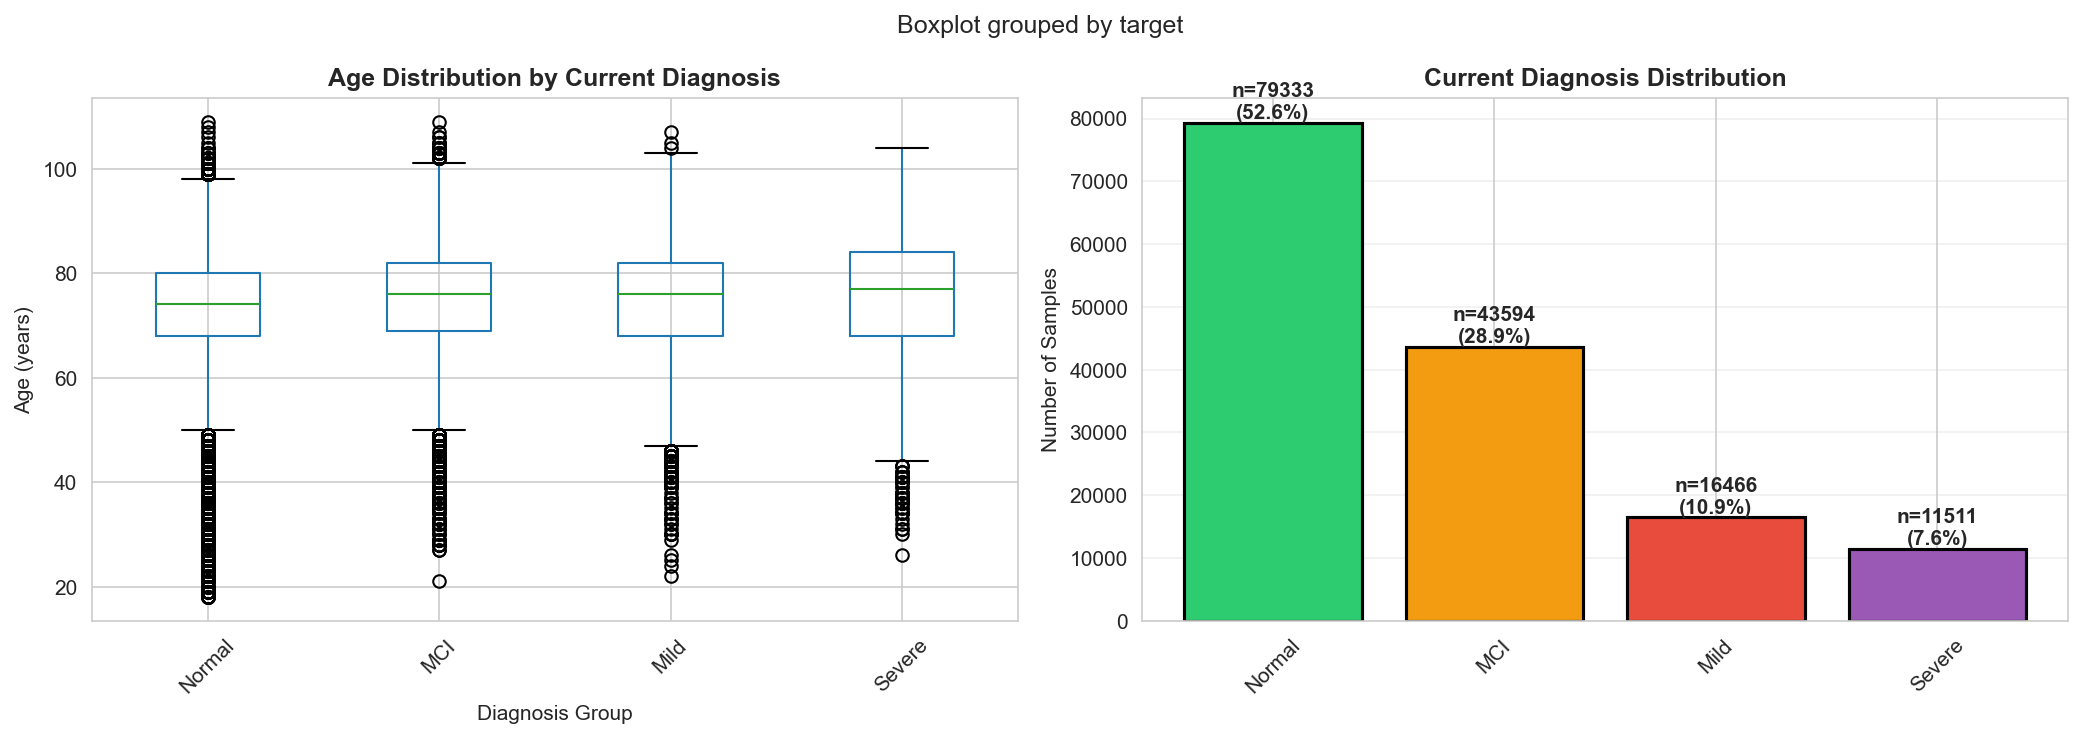
\includegraphics[width=0.95\columnwidth]{output/demographics_overview.png}}
\caption{Demographic characteristics of the study cohort. Left: Age distribution stratified by current diagnosis. Right: Class distribution showing natural imbalance.}
\label{fig:sup_demographics}
\end{figure}

\begin{figure*}[htbp]
\centerline{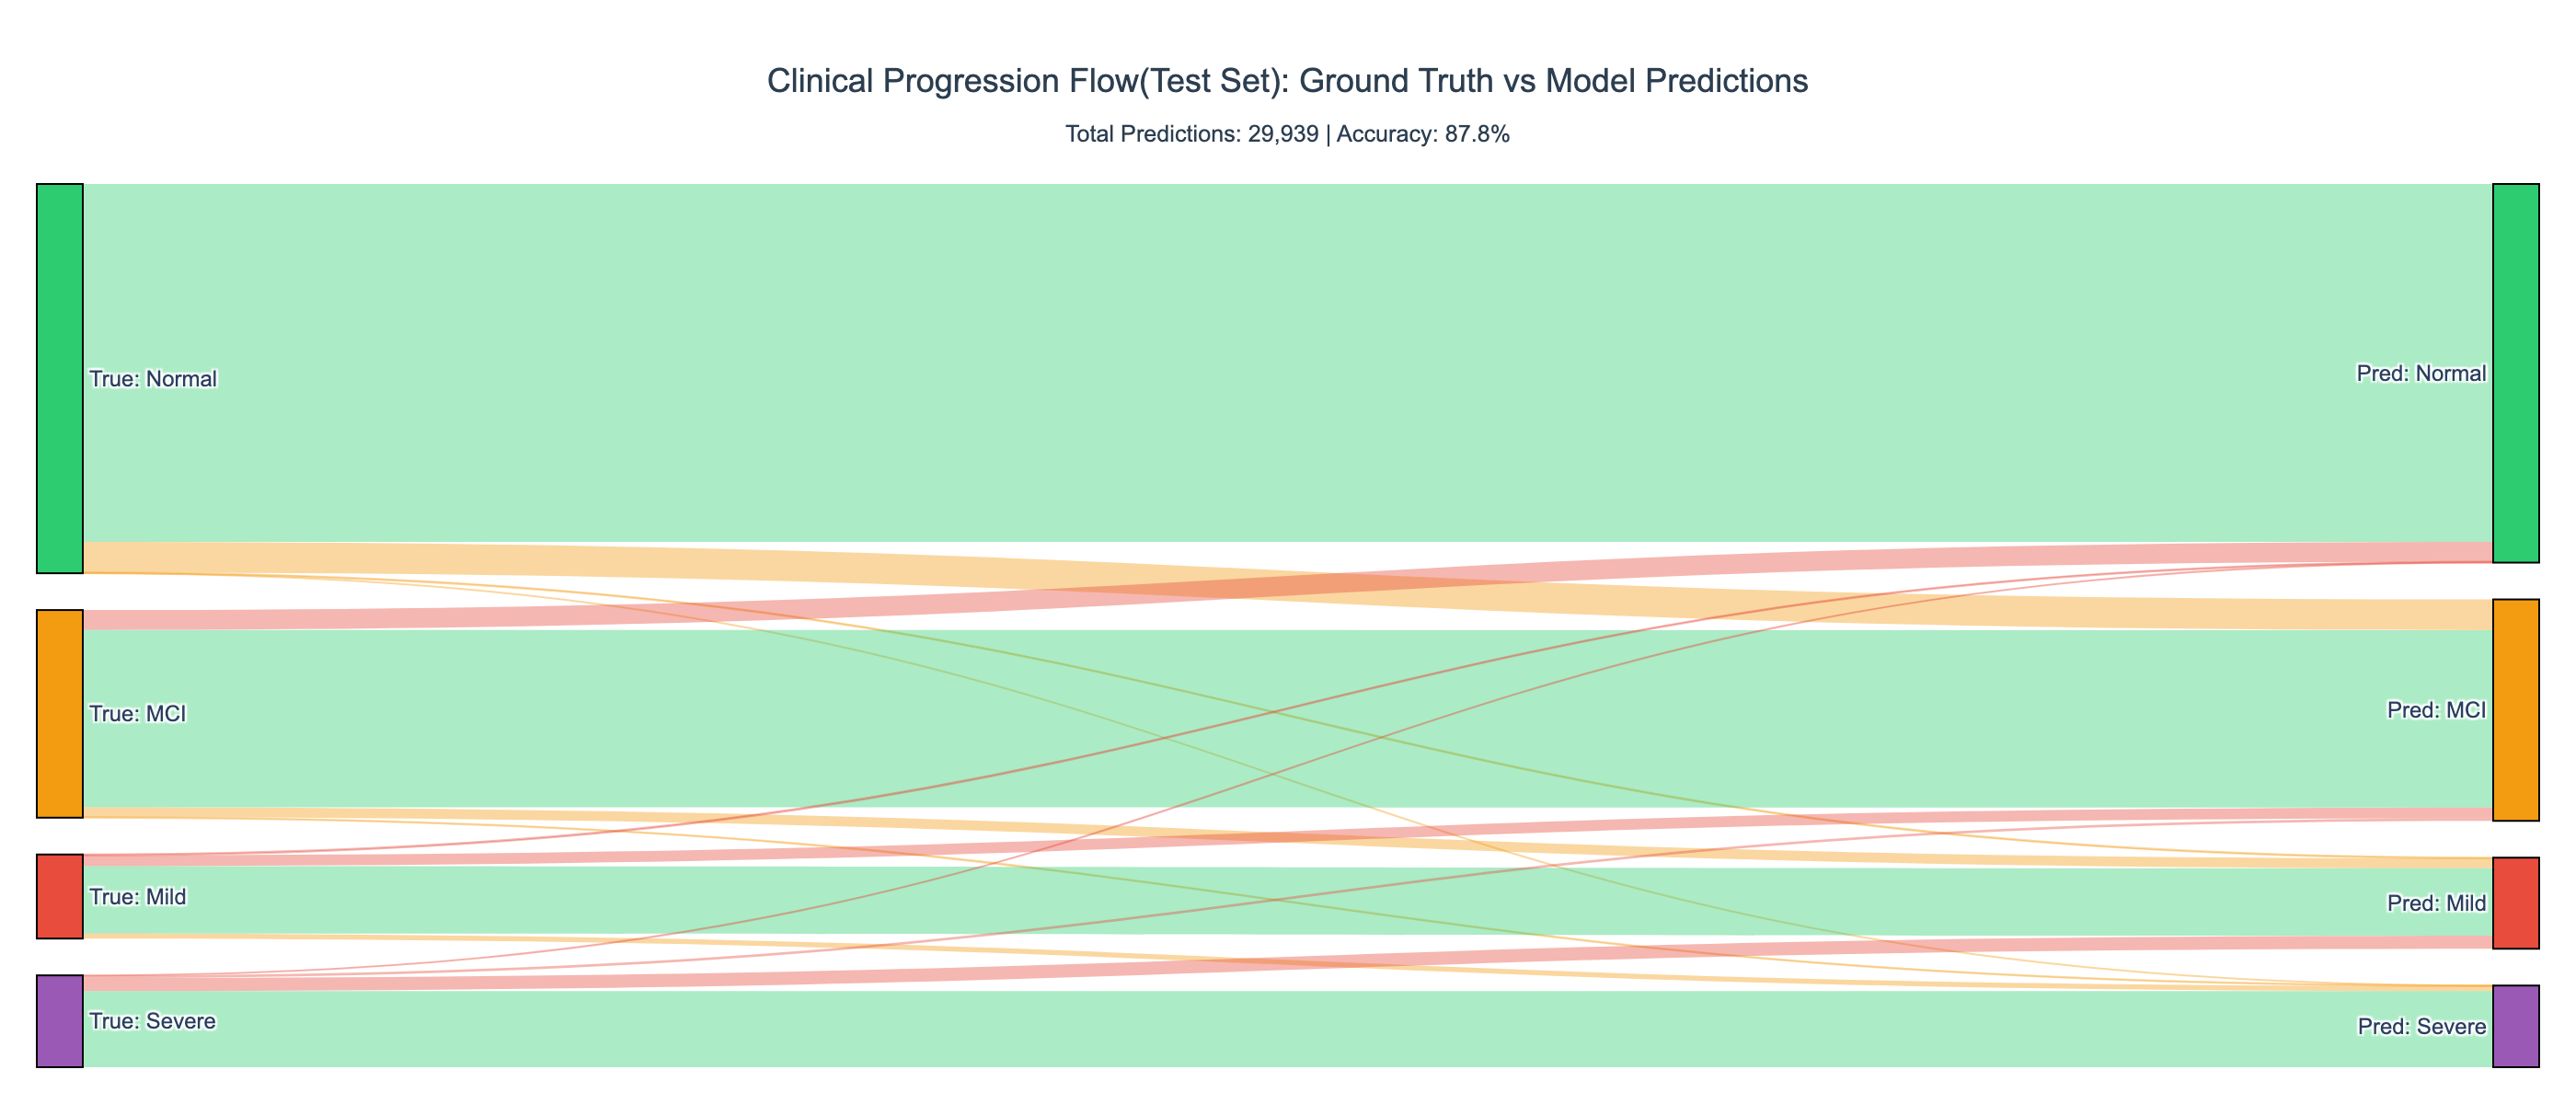
\includegraphics[width=0.85\textwidth]{output/sankey_progression_flow.png}}
\caption{Sankey Diagram of Clinical Progression (Test Set). Flow widths are proportional to patient counts. Left: True diagnosis at current visit. Right: Model-predicted diagnosis at subsequent visit.}
\label{fig:sup_sankey}
\end{figure*}

\begin{figure}[htbp]
\centerline{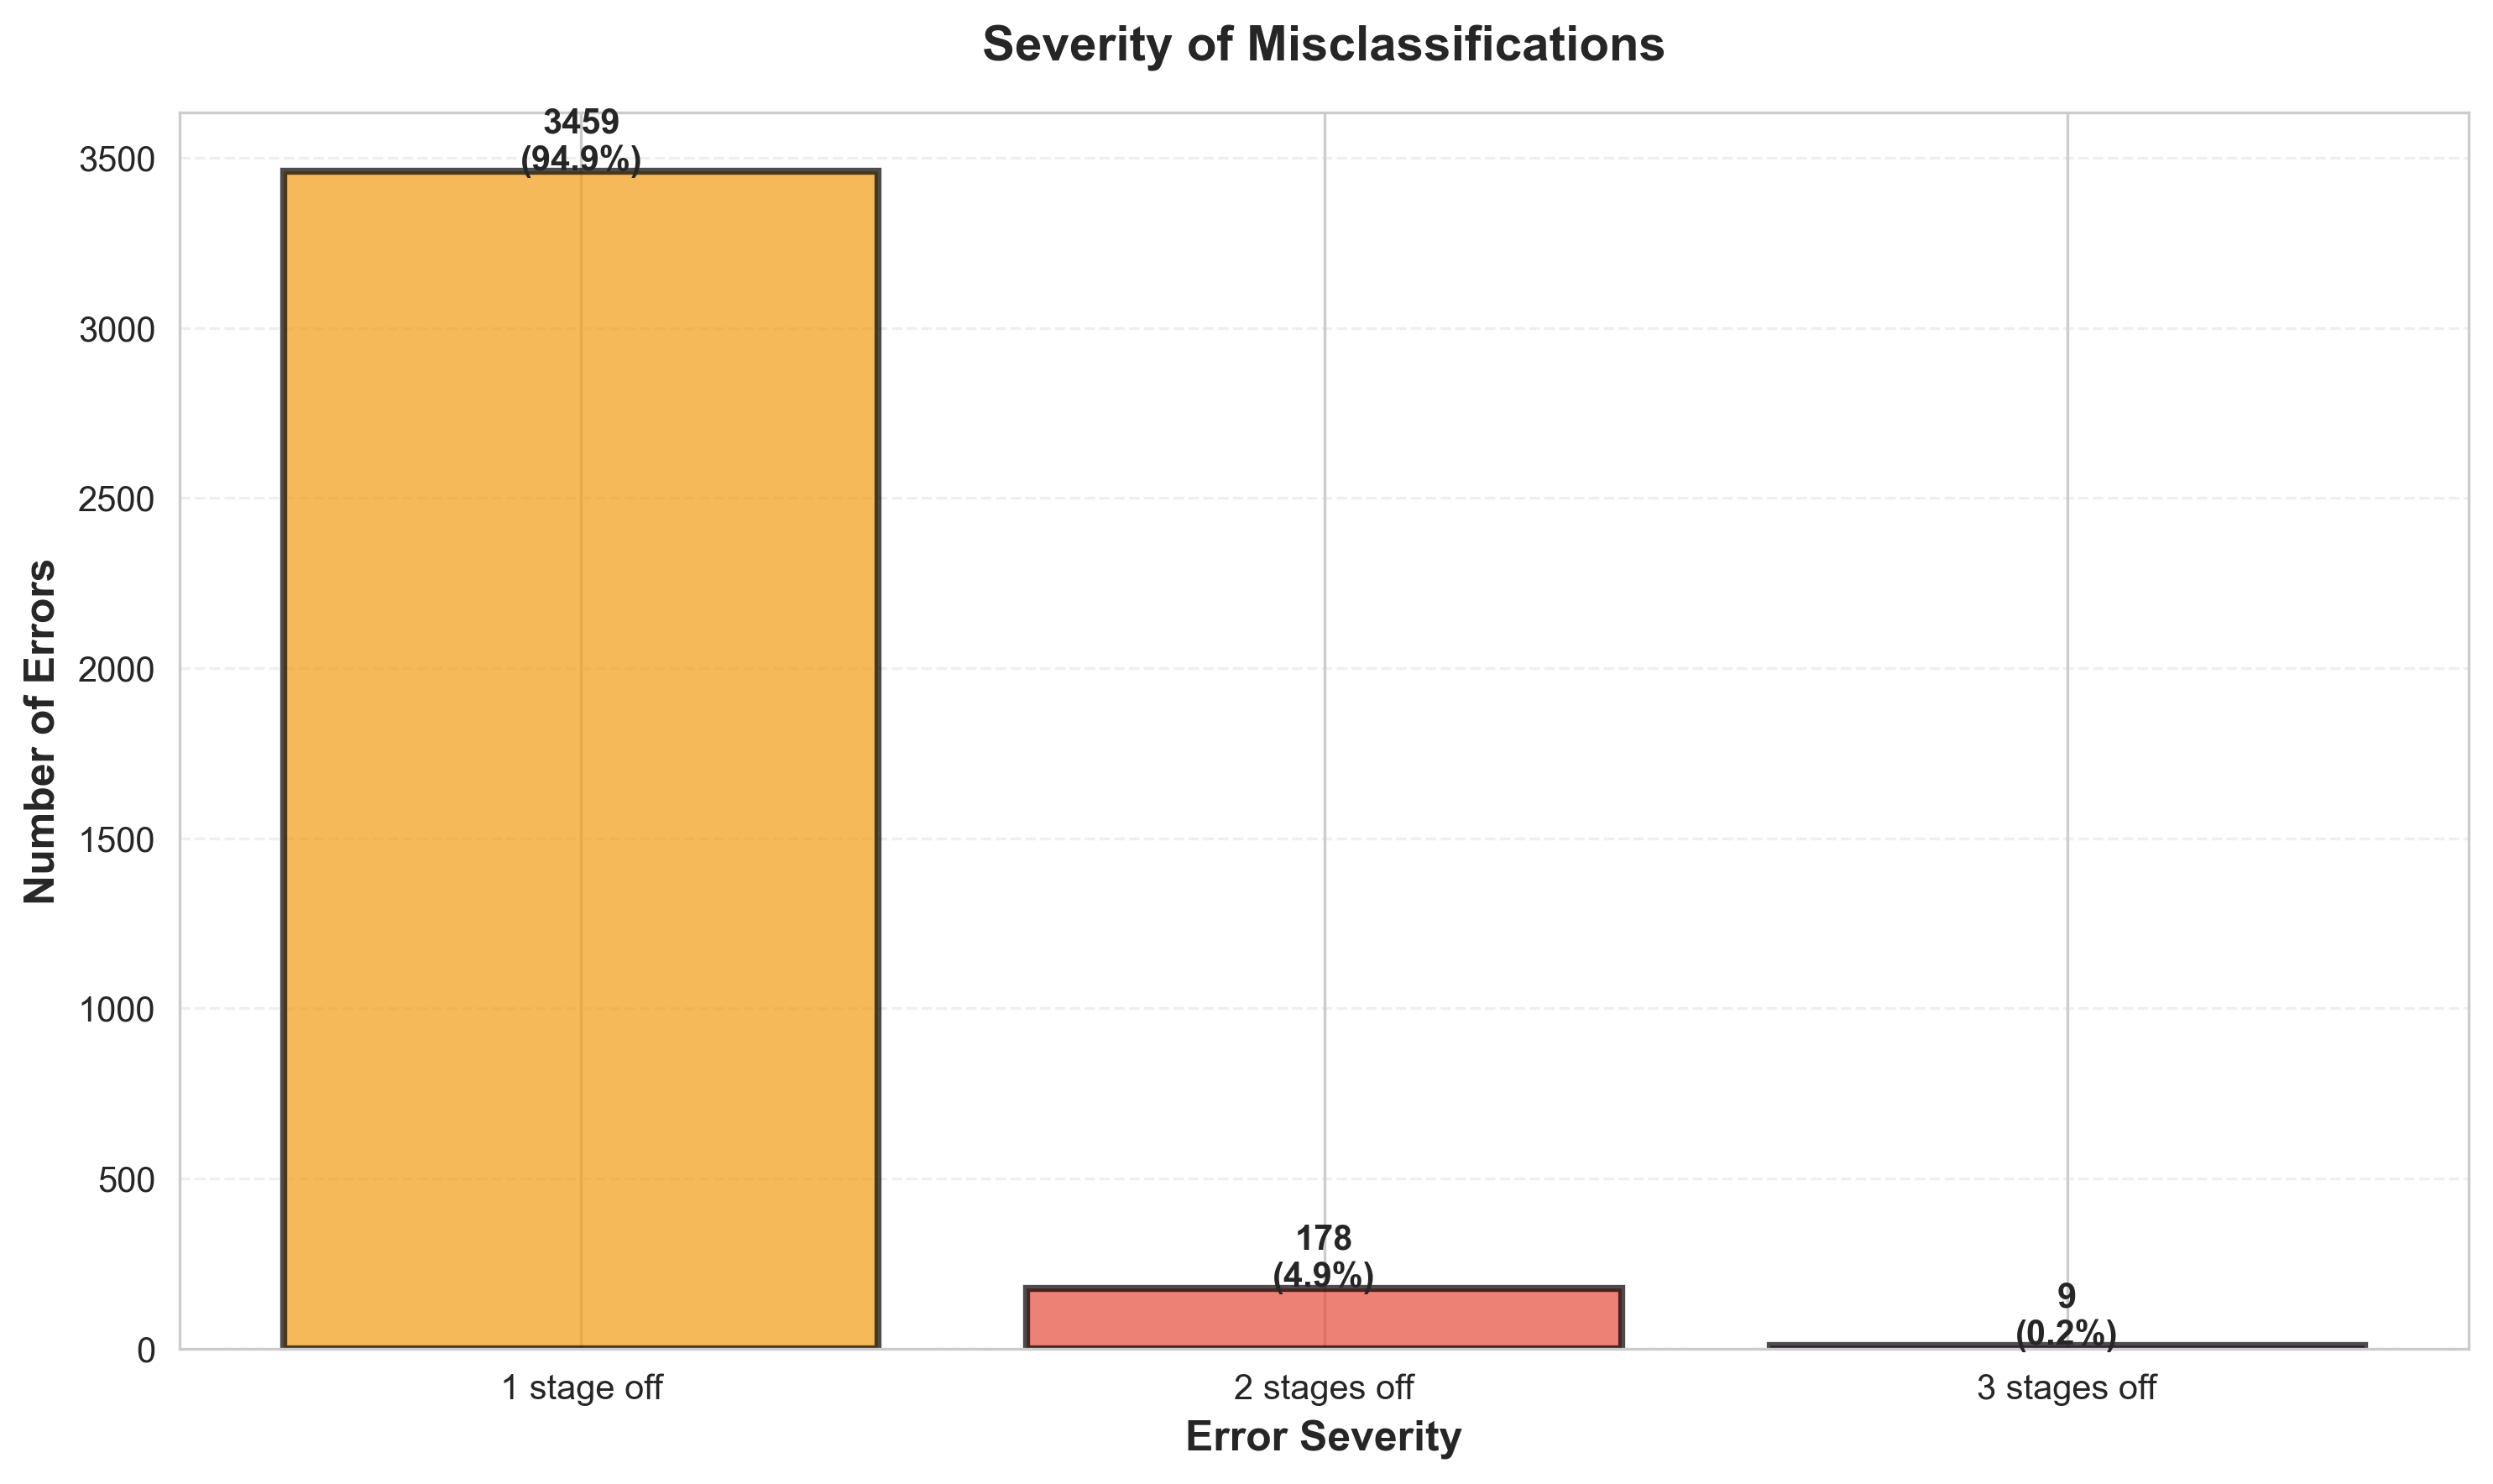
\includegraphics[width=0.9\columnwidth]{output/error_severity.png}}
\caption{Error Severity Analysis. Most errors are one stage off, indicating clinically proximal predictions.}
\label{fig:sup_severity}
\end{figure}

\begin{figure}[htbp]
\centerline{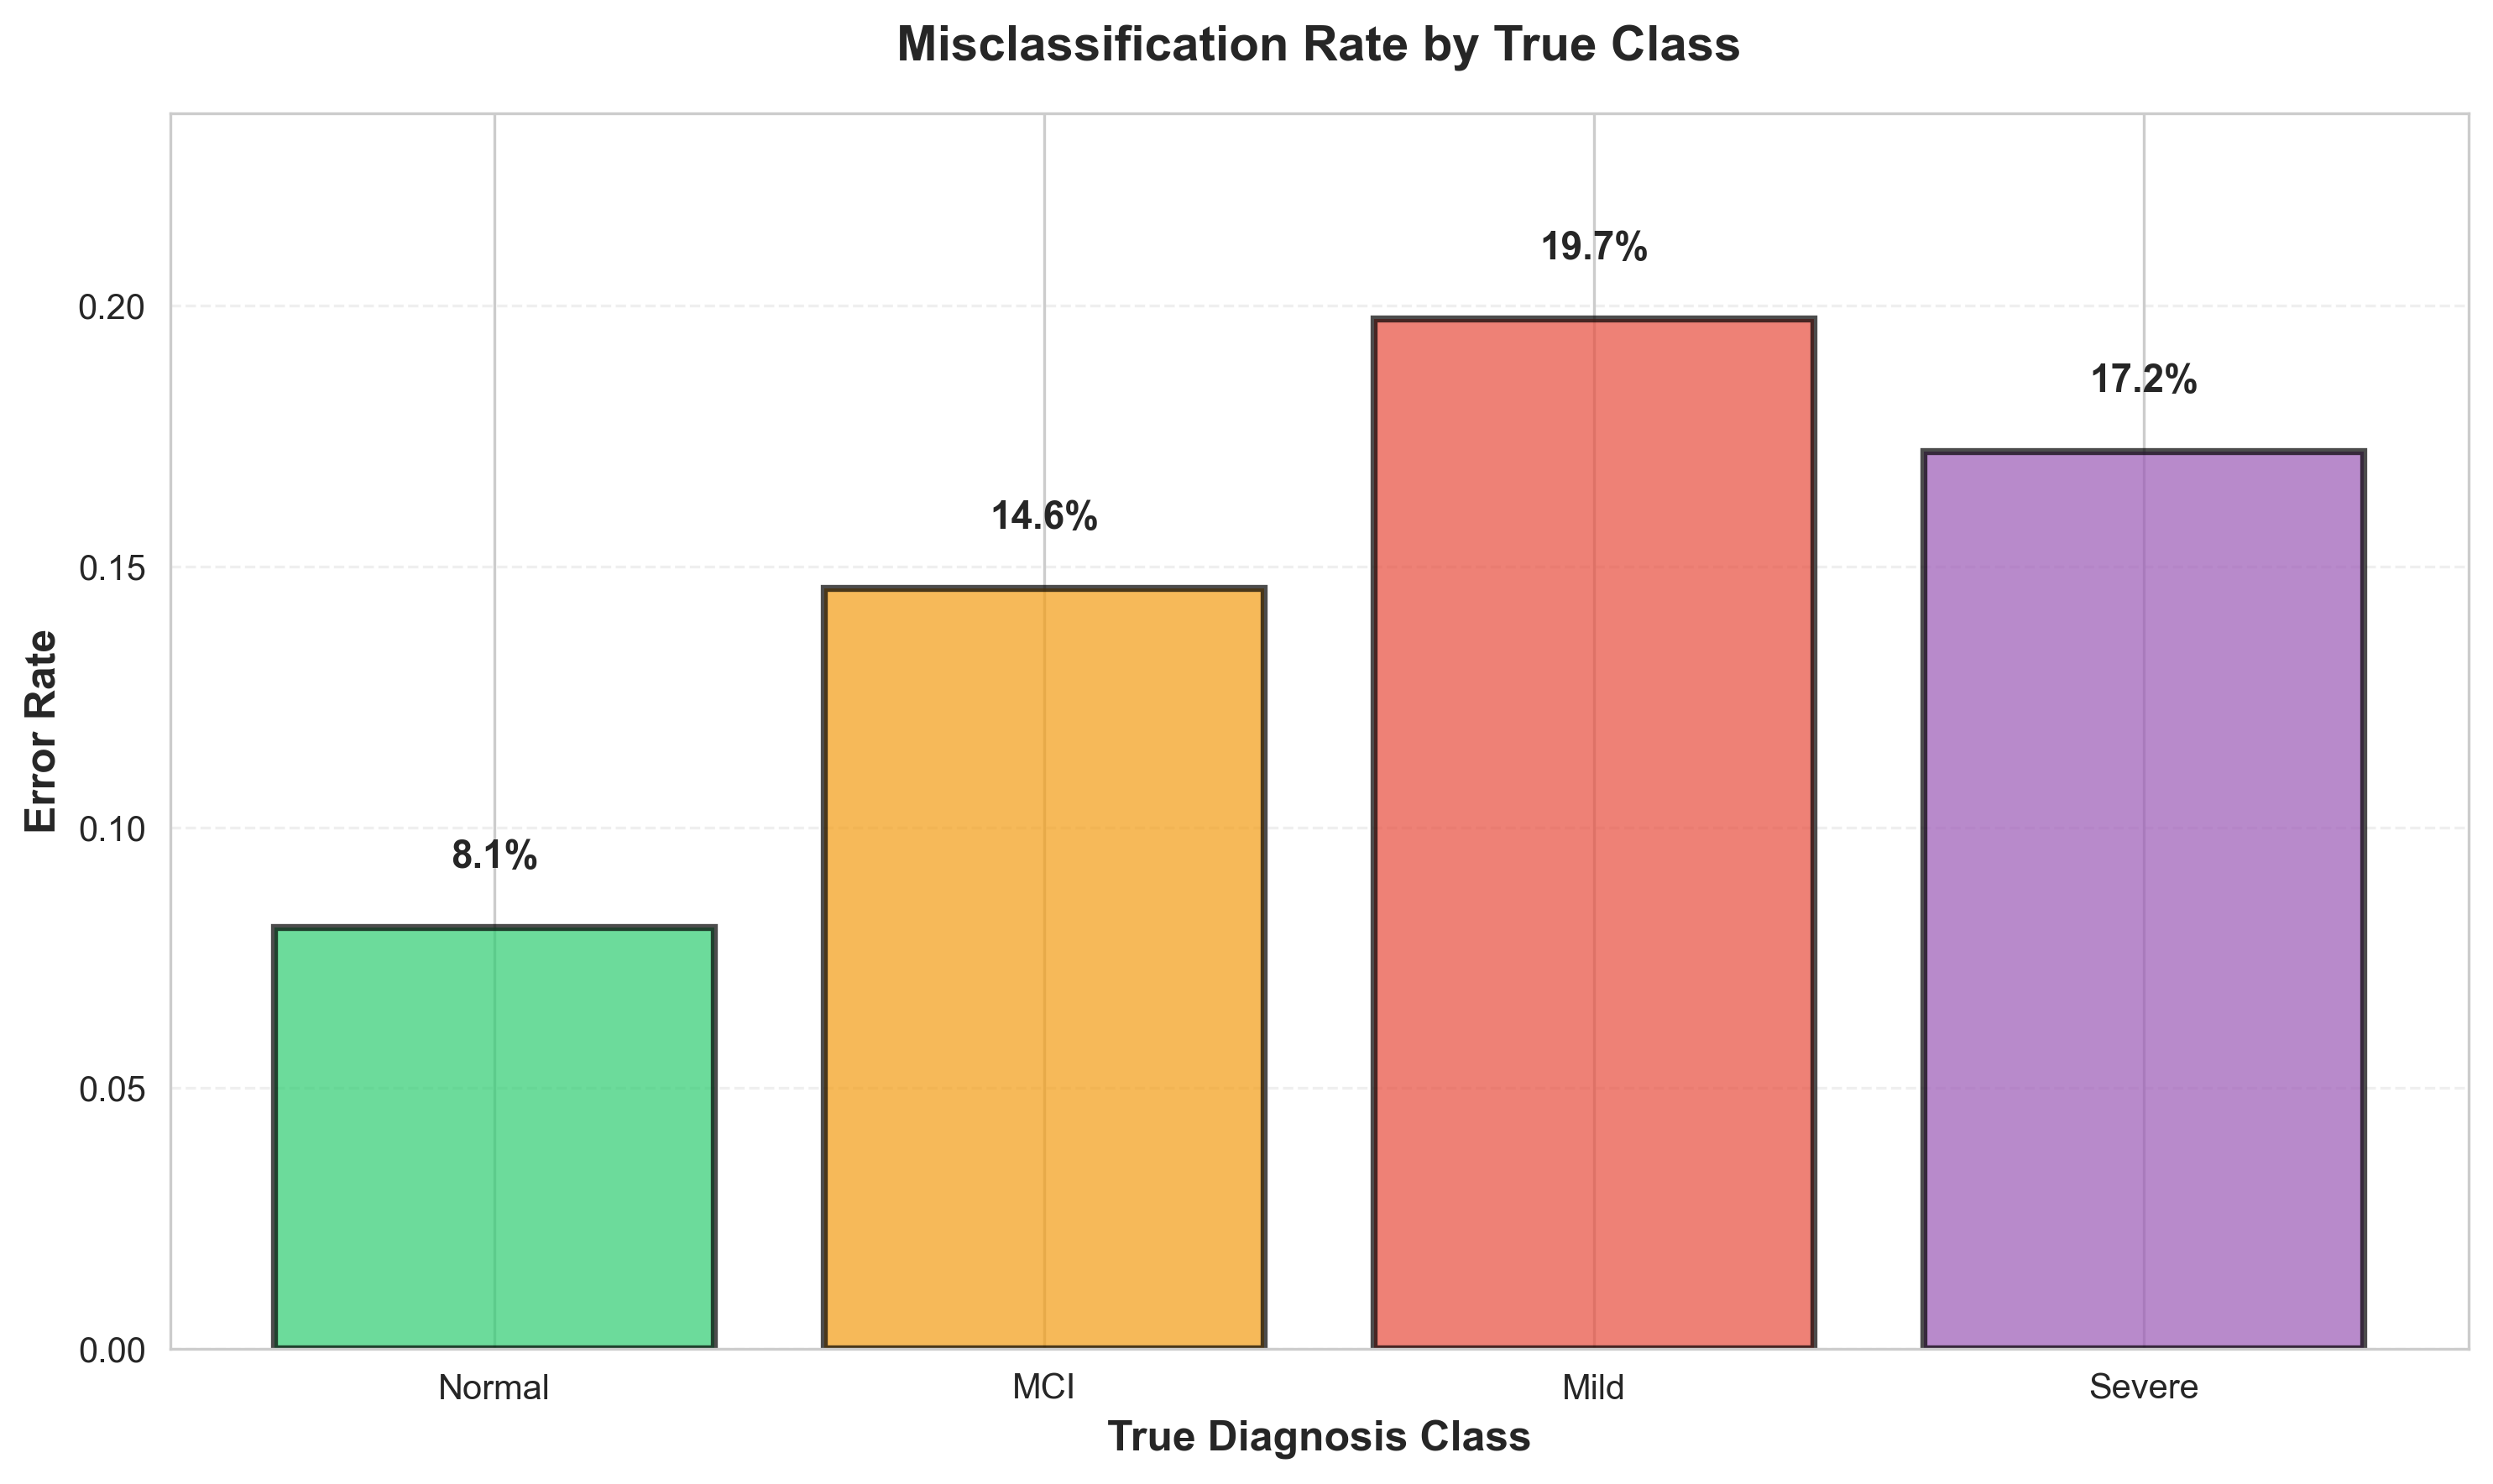
\includegraphics[width=0.9\columnwidth]{output/error_rate_by_class.png}}
\caption{Error Rate by True Class. The Mild dementia class has the highest observed error rate.}
\label{fig:sup_error_rate}
\end{figure}

\begin{figure}[htbp]
\centerline{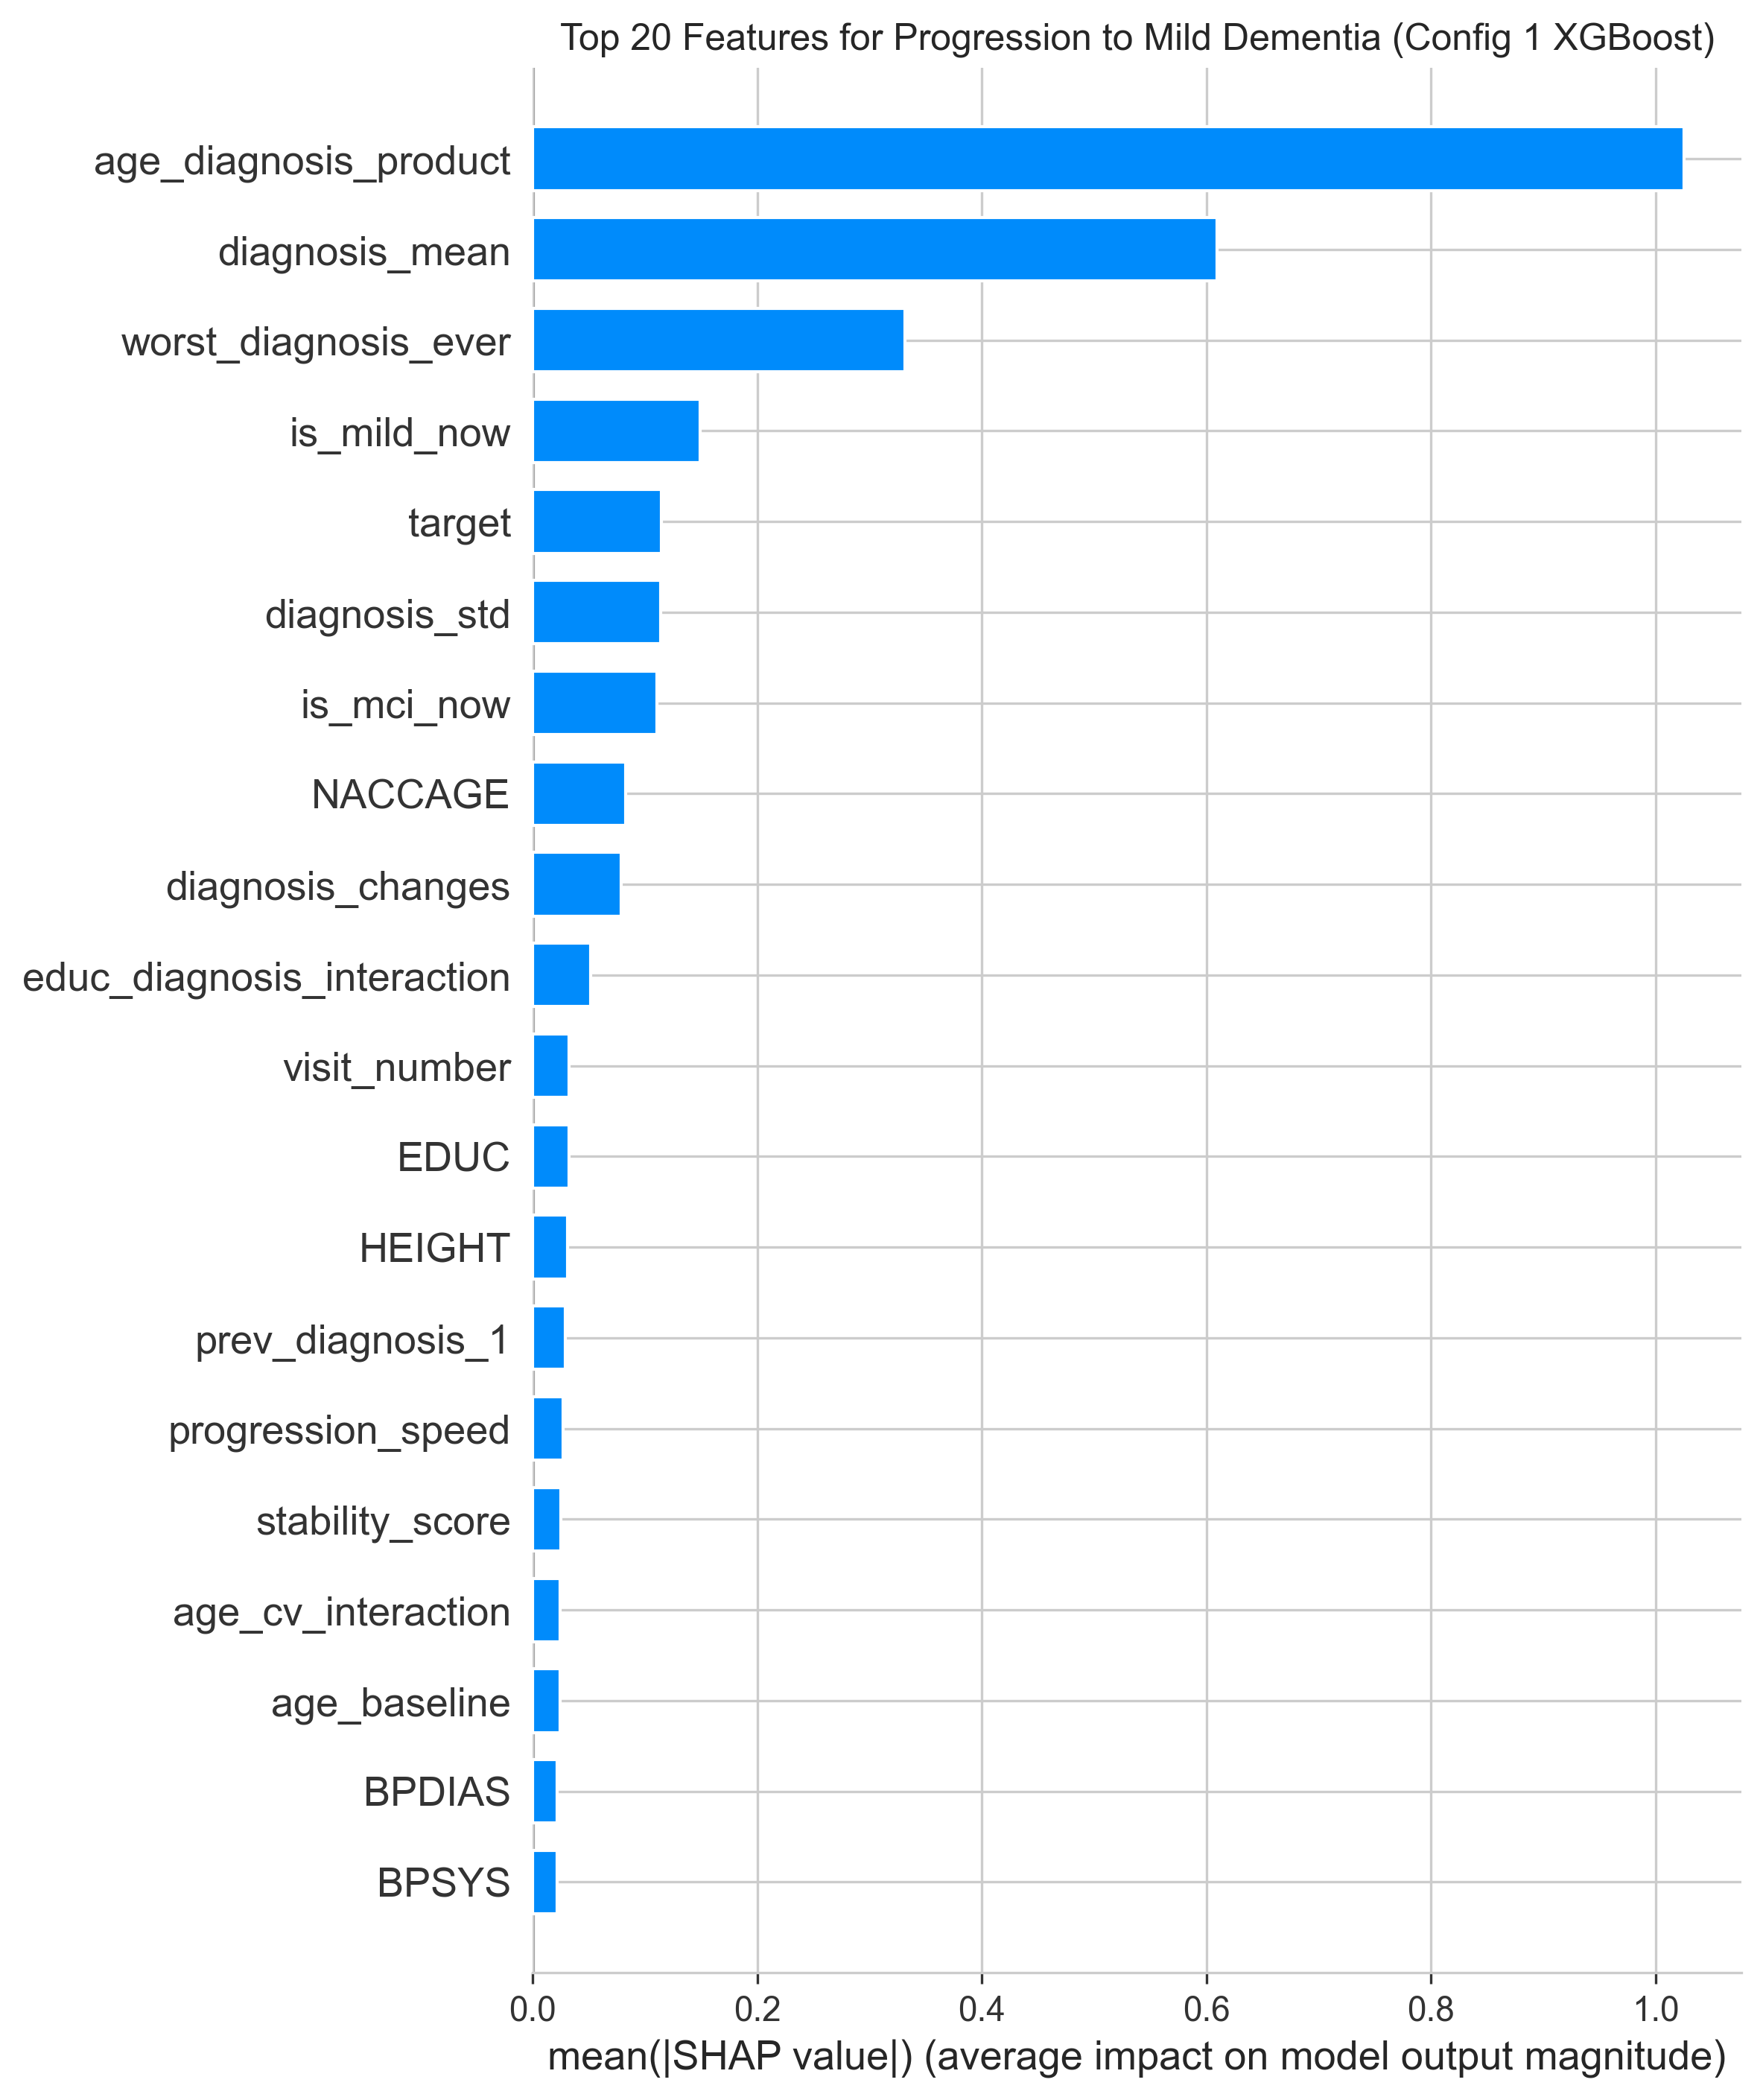
\includegraphics[width=0.95\columnwidth]{output/shap_importance_bar.png}}
\caption{SHAP Feature Importance Bar Chart. Mean absolute SHAP values quantify each feature's contribution to model predictions.}
\label{fig:sup_shap_bar}
\end{figure}

\begin{figure}[htbp]
\centerline{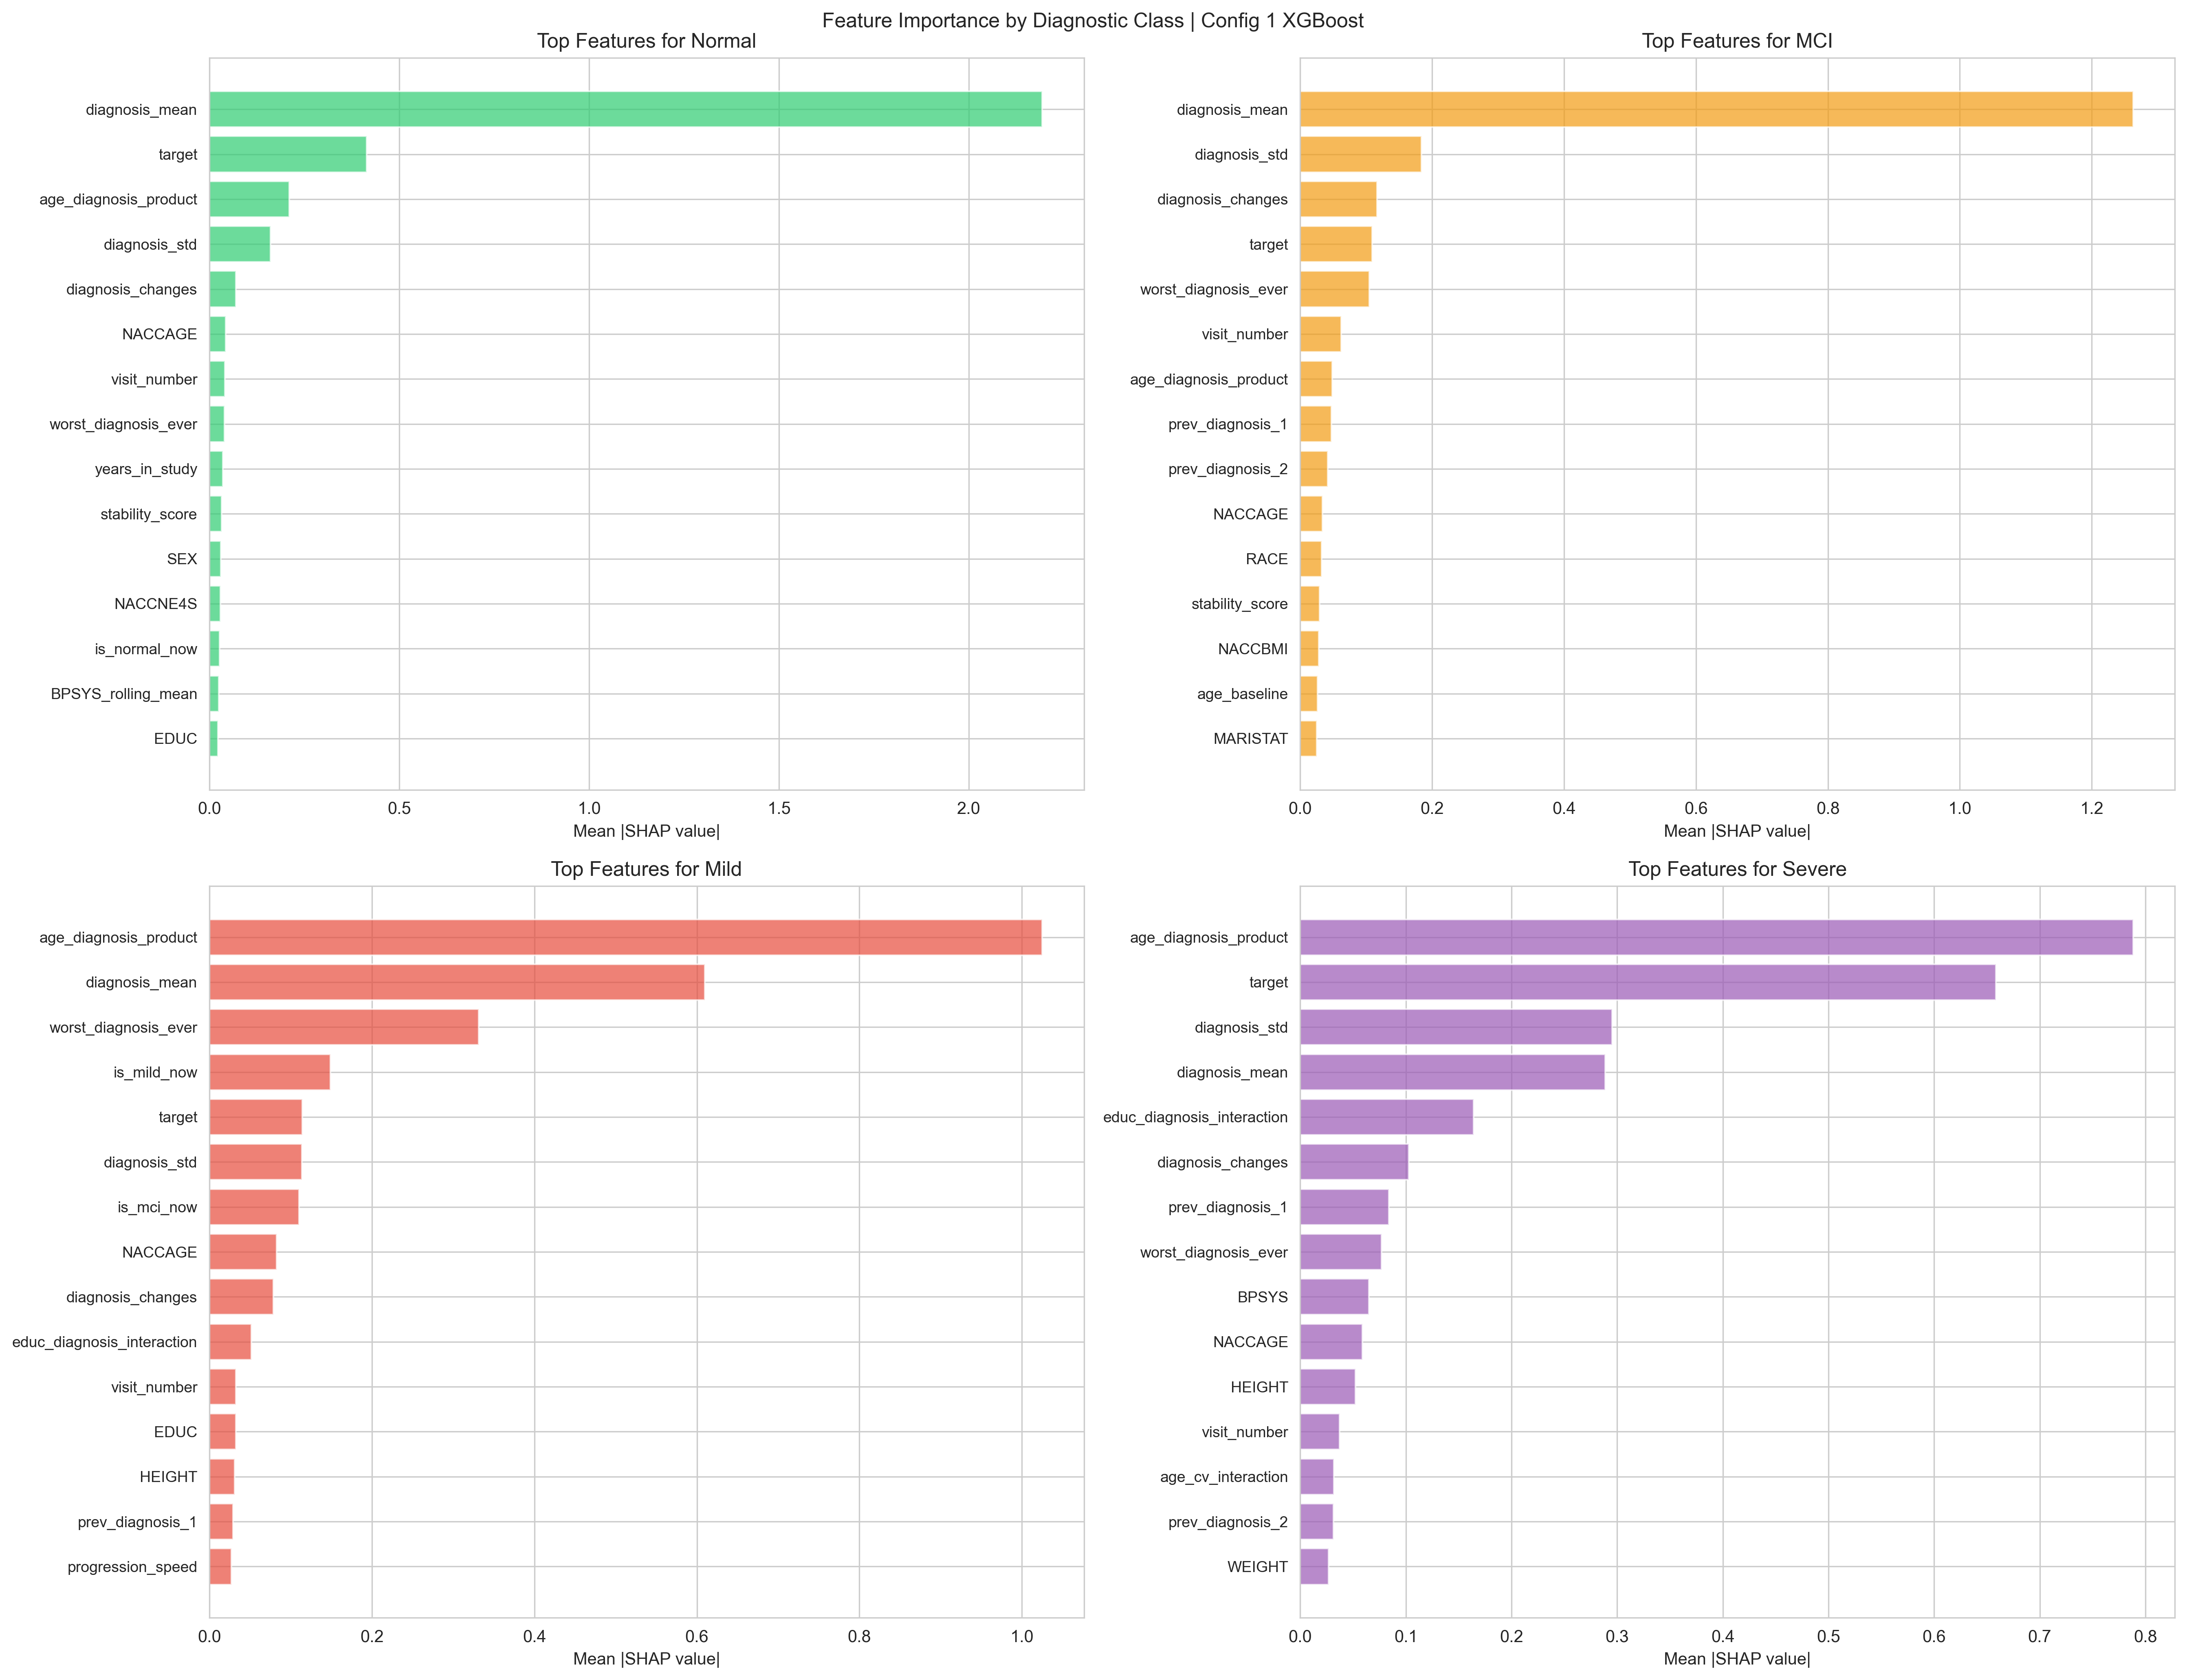
\includegraphics[width=0.95\columnwidth]{output/shap_all_classes.png}}
\caption{SHAP Feature Importance by Diagnostic Class. Each subplot shows the top contributing features for a diagnostic class.}
\label{fig:sup_shap_all}
\end{figure}

\begin{figure}[htbp]
\centerline{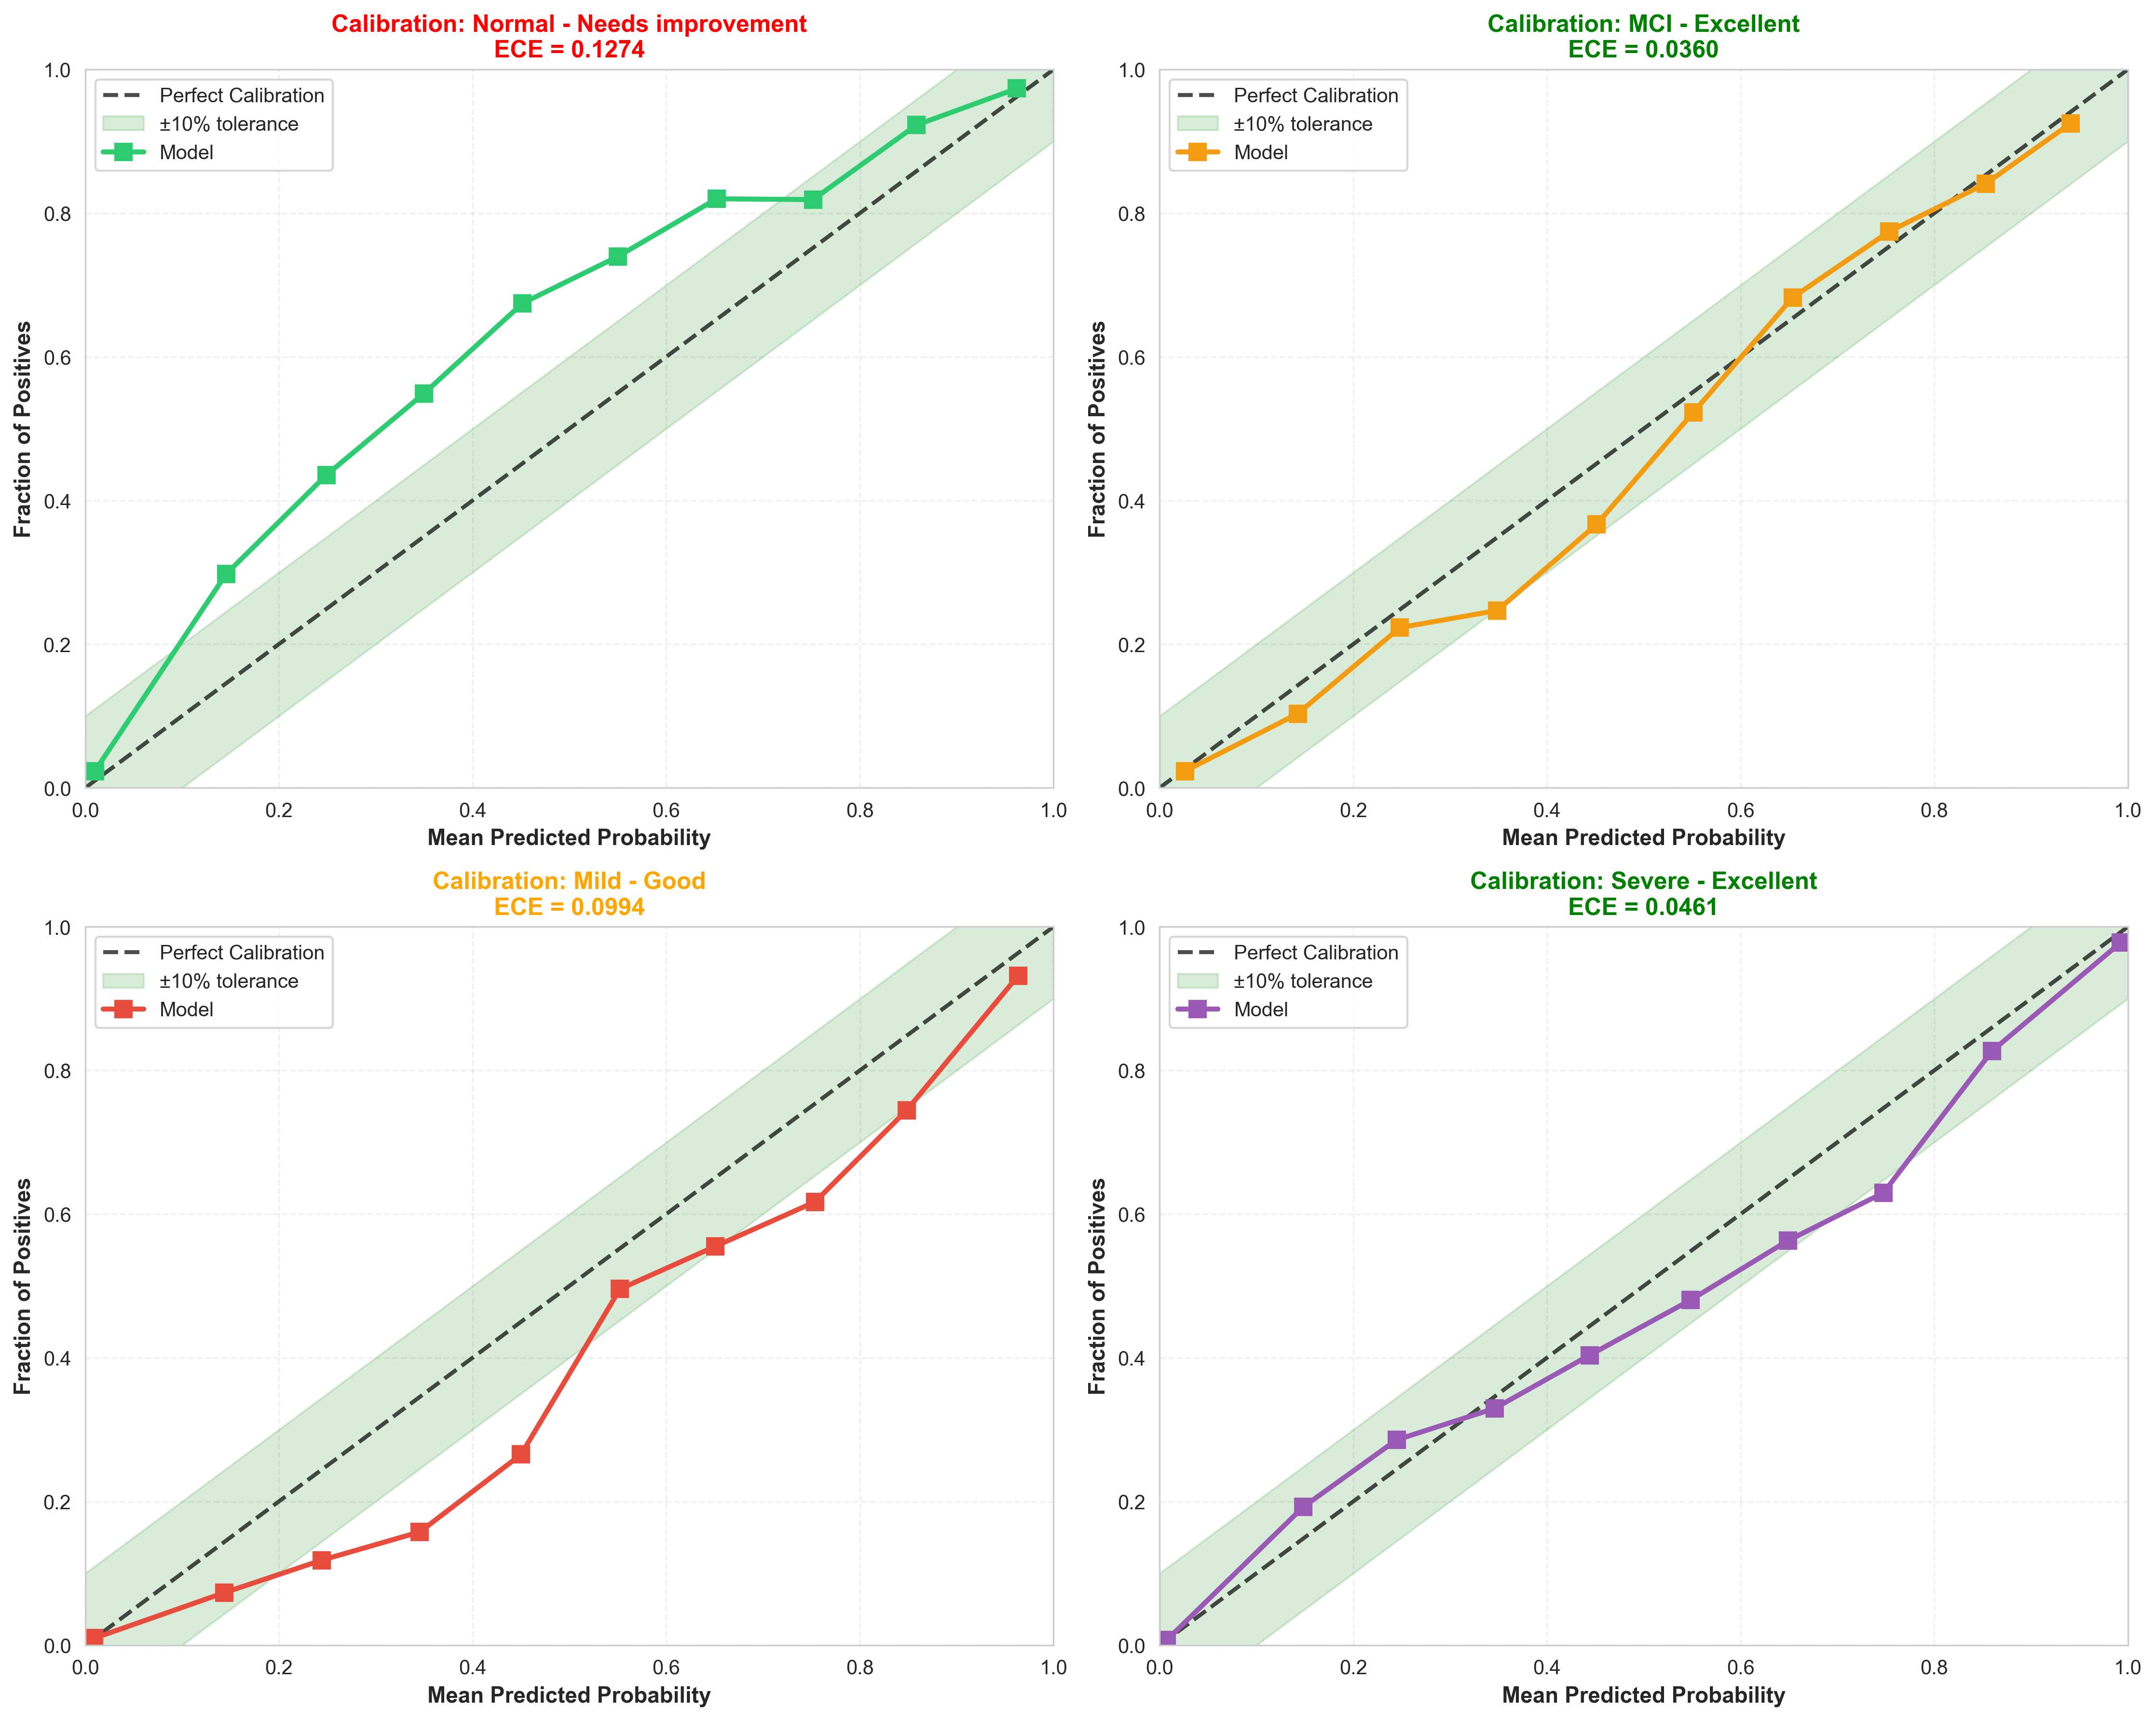
\includegraphics[width=0.9\columnwidth]{output/calibration_curves.png}}
\caption{Calibration Curves by Class. ECE values are 0.3643 (Normal), 0.3382 (MCI), 0.3528 (Mild), and 0.3225 (Severe).}
\label{fig:sup_calibration}
\end{figure}

\begin{figure}[htbp]
\centerline{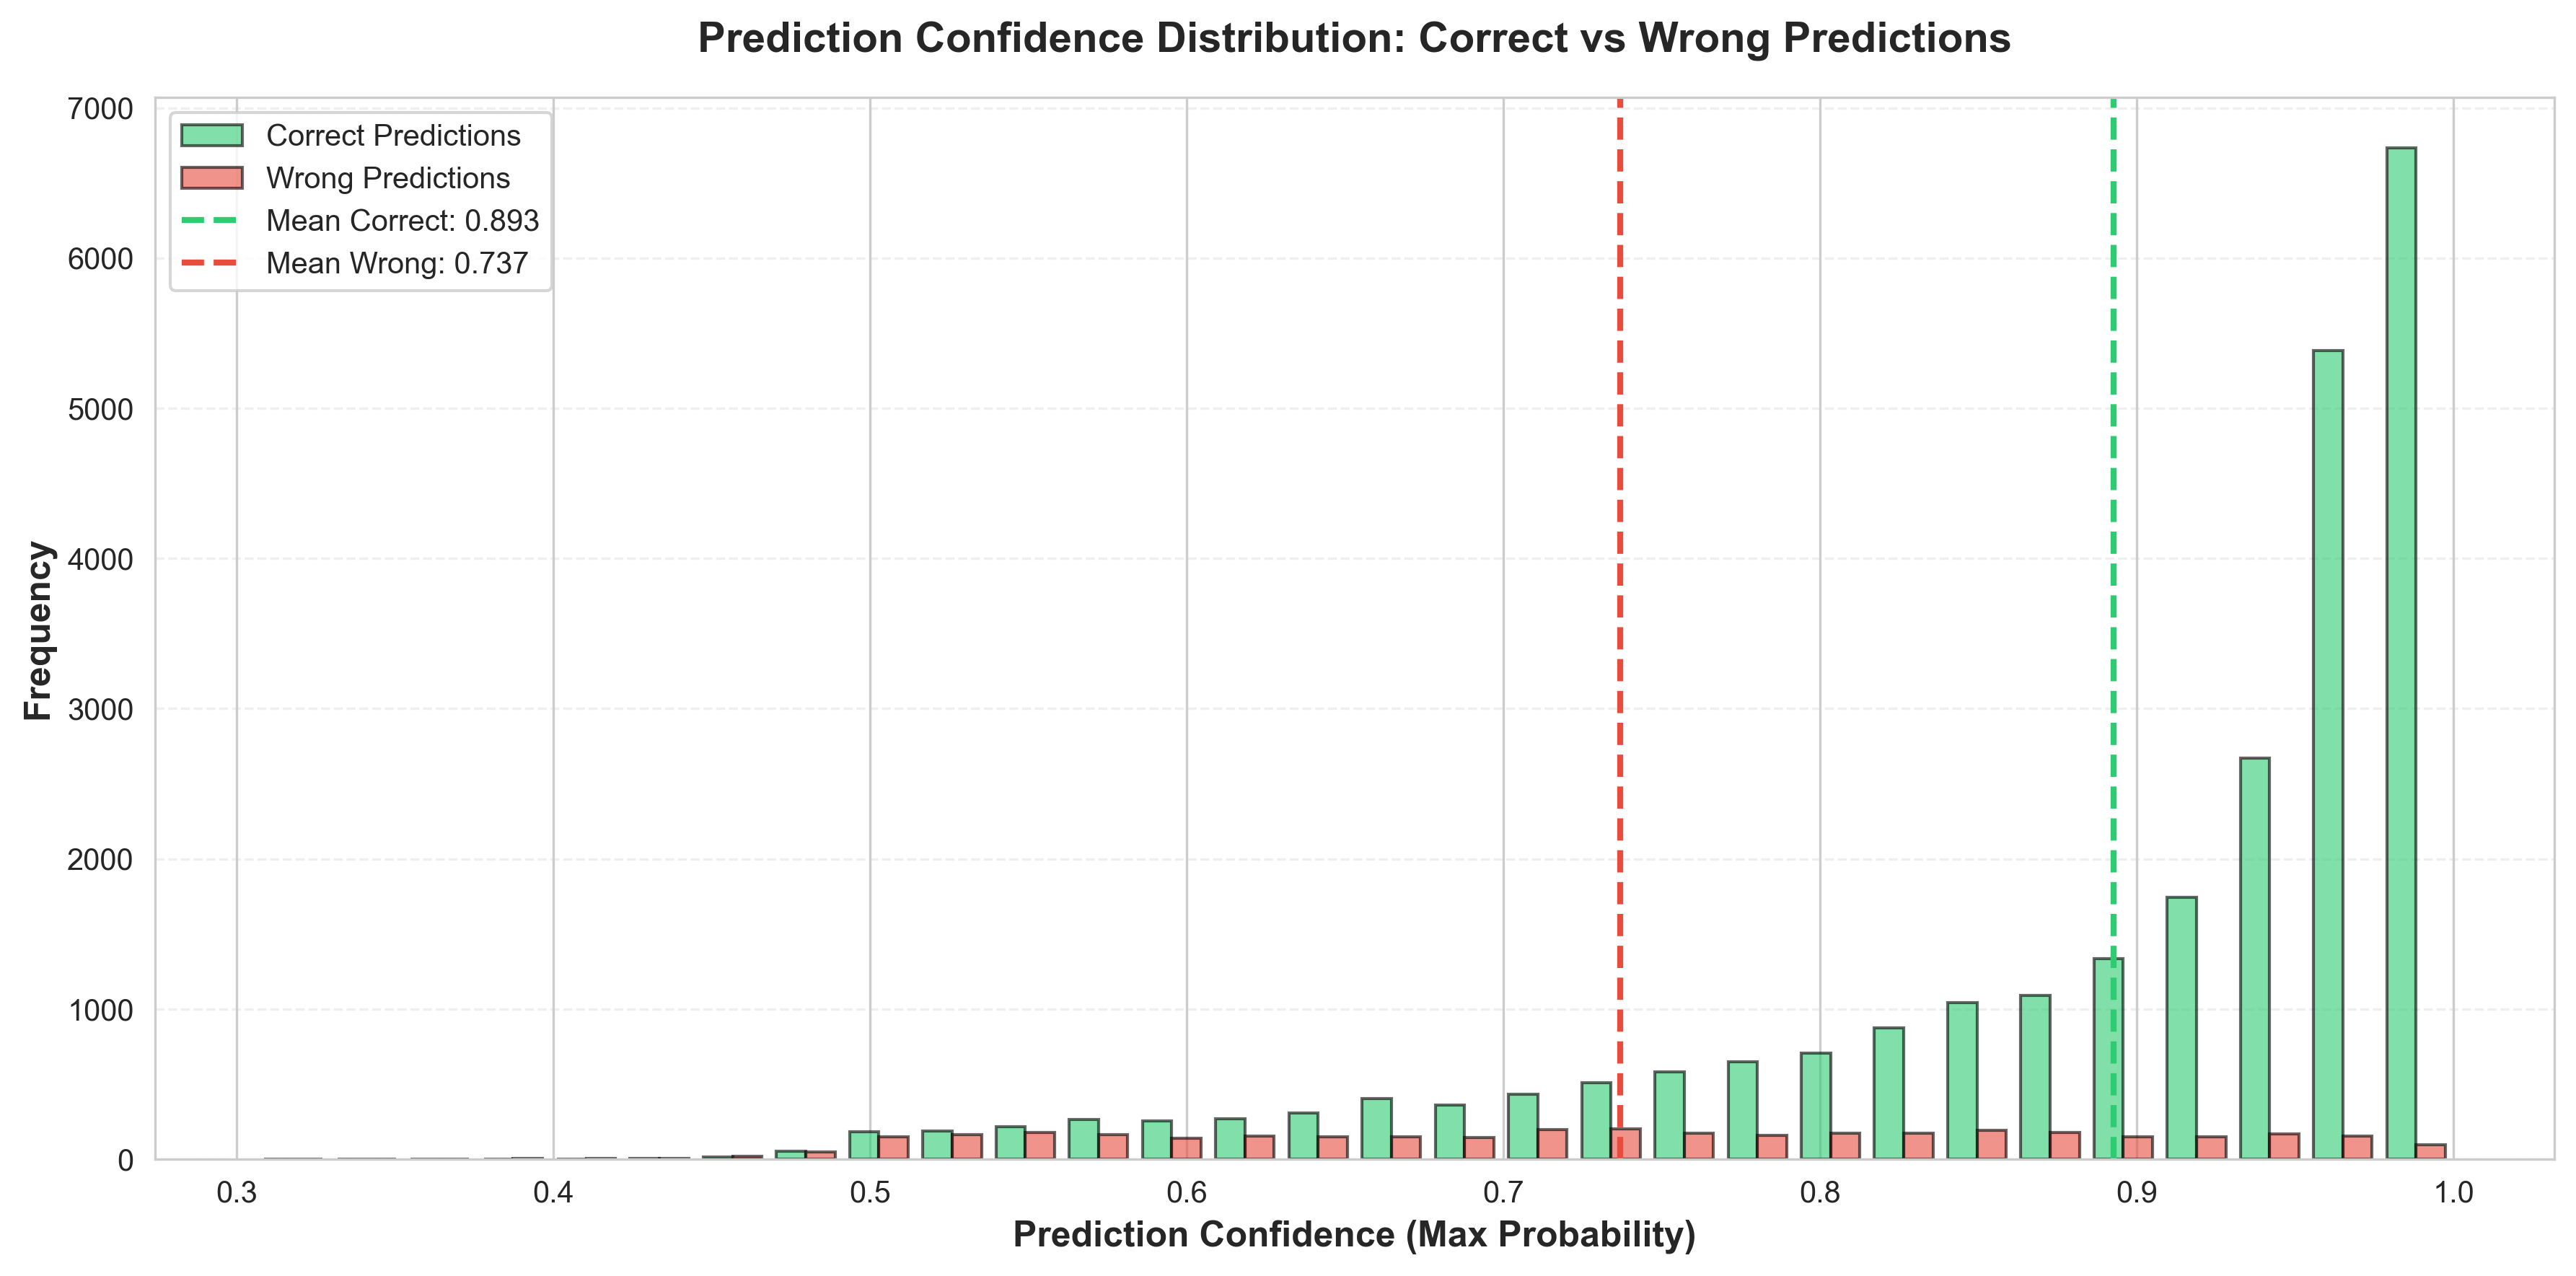
\includegraphics[width=0.9\columnwidth]{output/confidence_analysis.png}}
\caption{Confidence Distribution Analysis. Correct predictions have mean maximum probability 0.319 versus 0.261 for incorrect predictions.}
\label{fig:sup_confidence}
\end{figure}

\begin{table}[htbp]
\caption{Ablation Study: Model Complexity vs Performance.}
\label{tab:sup_ablation}
\begin{center}
\begin{tabular}{lccc}
\toprule
\textbf{Configuration} & \textbf{Accuracy} & \textbf{F1-Macro} & \textbf{Complexity} \\
\midrule
\textbf{Base XGBoost} & \textbf{0.8859} & \textbf{0.8557} & \textbf{Low} \\
XGBoost + SMOTE & 0.8818 & 0.8486 & Medium \\
Full Ensemble + SMOTE & 0.8704 & 0.8390 & High \\
\bottomrule
\end{tabular}
\end{center}
\end{table}

\end{document}
